
%% Harvard Physics Project
%% Test Booklet 5: Models of the Atom
%%--------------------------------------------------


%% Test Booklet 5 contains 70 - 3 questions


%% Test A
%%--------------------
\element{project}{
\begin{question}{testA-Q01}
    Which one of the following equations relates an increase
        in an object's mass with an increase in the object's speed?
    %% NOTE: I personally dislike this definition of mass
    %% NOTE:  E^2 = m^2 + p^2
    \begin{multicols}{2}
    \begin{choices}
        \wrongchoice{$m = \dfrac{F}{m}$}
        \wrongchoice{$\dfrac{q}{m} = \dfrac{v}{BR}$}
        \wrongchoice{$\dfrac{1}{2} = hf - W$}
      \correctchoice{$m = \dfrac{m_0}{\sqrt{1-\dfrac{v^2}{c^2}}}$}
        \wrongchoice{$mv = \dfrac{hf}{c}$}
    \end{choices}
    \end{multicols}
\end{question}
}

\element{project}{
\begin{questionmult}{testA-Q02}
    Which of the following could not be explained in terms of classical physics?
    \begin{choices}
      \correctchoice{the photoelectric effect}
      \correctchoice{variation of mass with speed}
      \correctchoice{the Compton effect}
    \end{choices}
\end{questionmult}
}

\element{project}{
\begin{question}{testA-Q03}
    An electron from a hydrogen atom:
    \begin{choices}
      \correctchoice{is identical to an electron from an oxygen atom,}
        \wrongchoice{has greater rest mass than an electron from an oxygen atom.}
        \wrongchoice{is larger than an electron from an oxygen atom.}
        \wrongchoice{has greater charge than an electron from an oxygen atom.}
    \end{choices}
\end{question}
}

\element{project}{
\begin{question}{testA-Q04}
    A reasonable prediction,
        based on the evolution of previous scientific theories,
        is that in the future the quantum theory will:
    \begin{choices}
        \wrongchoice{be replaced by a theory based on a mechanical model.}
      \correctchoice{be replaced by a more general theory.}
        \wrongchoice{be shown to be wrong.}
        \wrongchoice{explain everything about nature.}
    \end{choices}
\end{question}
}

\element{project}{
\begin{questionmult}{testA-Q05}
    A clean surface of potassium metal will emit
        electrons when exposed to blue light.
    If the intensity of the blue light is increased,
        which of the following will increase also?
    \begin{choices}
      \correctchoice{the number of electrons ejected per second}
        \wrongchoice{the maximum kinetic energy of the ejected electrons}
        \wrongchoice{the charge of each ejected electron}
    \end{choices}
\end{questionmult}
}

\element{project}{
\begin{question}{testA-Q06}
    %% NOTE: formating of fractions??
    In an electrolysis experiment, a certain amount of hydrogen is collected.
    If the experiment were repeated with 1/3 as much electric current,
        and 1/5 as much time, how much hydrogen would be collected?
    \begin{multicols}{2}
    \begin{choices}
      \correctchoice{\num{1/15} as much}
        \wrongchoice{\num{1/8} as much}
        \wrongchoice{\num{1/5} as much}
        \wrongchoice{\num{1/3} as much}
        \wrongchoice{\num{1/2} as much}
    \end{choices}
    \end{multicols}
\end{question}
}

\element{project}{
\begin{question}{testA-Q07}
    \emph{All except one} of the following terms can be applied
        to both an x-ray and an atom of hydrogen.
    Find the exception.
    \begin{multicols}{2}
    \begin{choices}
        \wrongchoice{wavelength}
        \wrongchoice{momentum}
        \wrongchoice{velocity}
      \correctchoice{rest mass}
        \wrongchoice{energy}
    \end{choices}
    \end{multicols}
\end{question}
}

\element{project}{
\begin{question}{testA-Q08}
    Bohr's atomic model:
    \begin{choices}
      \correctchoice{allows only certain values of angular momenta
            for the orbital electron of hydrogen.}
        \wrongchoice{explains the spectra of elements whose atoms
            have more than one electron in the outermost shell.}
        \wrongchoice{assumes that electrons have wave properties.}
    \end{choices}
\end{question}
}

\element{project}{
\begin{question}{testA-Q09}
    In the modem periodic table,
        the elements are arranged in order of increasing:
    \begin{choices}
        \wrongchoice{atomic mass.}
      \correctchoice{atomic number.}
    \end{choices}
\end{question}
}

\element{project}{
\begin{questionmult}{testA-Q10}
    Which of the following entered significantly into the
        determination of $\dfrac{q}{m}$ for electrons in
        Joseph John ``J. J.'' Thomson's experiment?
    \begin{choices}
        \wrongchoice{A force acts upon a moving electron in a gravitational field.}
        %% NOTE: must use both electric and magnetic deflection
      \correctchoice{A force acts upon a moving electron in an electric field.}
      \correctchoice{A force acts upon a moving electron in a magnetic field.}
    \end{choices}
\end{questionmult}
}

\element{project}{
\begin{question}{testA-Q11}
    In a scattering experiment,
        some alpha particles directed towards a gold foil come straight back.
    At the point of closest approach of an alpha particle to the nucleus of the gold atom,
        the alpha particle must have had zero:
    \begin{choices}
      \correctchoice{kinetic energy.}
        \wrongchoice{potential energy.}
        \wrongchoice{electrical energy.}
        \wrongchoice{acceleration.}
        \wrongchoice{charge.}
    \end{choices}
\end{question}
}

\element{project}{
\begin{question}{testA-Q12}
    A beam of electrons is directed between two charged
        plates as indicated in the diagram below.
    The upper plate is positively charged,
        while the lower plate is negatively charged.
    \begin{center}
    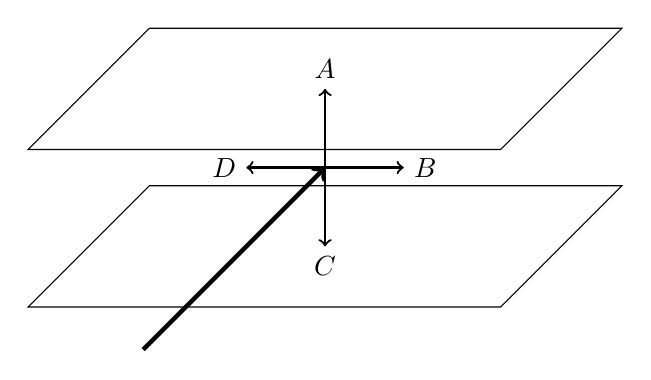
\begin{tikzpicture}
        %% NOTE: TODO: tikz, this is a 3D diagram
        %% draw each plate
        \foreach \y in {-1,1} 
            \draw (-3,\y,2) -- (3,\y,2) -- (3,\y,-2) -- (-3,\y,-2) -- cycle;
        %% incoming vector
        \draw[ultra thick,->] (0,0,6) -- (0,0,0); 
        %% outgoing vectors
        \draw[thick,->] (0,0,0) -- (-1,0,0) node[anchor=east] {$D$};
        \draw[thick,->] (0,0,0) -- (+1,0,0) node[anchor=west] {$B$};
        \draw[thick,->] (0,0,0) -- (0,+1,0) node[anchor=south] {$A$};
        \draw[thick,->] (0,0,0) -- (0,-1,0) node[anchor=north] {$C$};
    \end{tikzpicture}
    \end{center}
    Once the beam is between the plates it will:
    \begin{choices}
        %% NOTE: opposites attract
      \correctchoice{curve in direction $A$.}
        \wrongchoice{curve in direction $B$.}
        \wrongchoice{curve in direction $C$.}
        \wrongchoice{curve in direction $D$.}
        \wrongchoice{continue in a straight line.}
    \end{choices}
\end{question}
}

\element{project}{
\begin{question}{testA-Q13}
    When the speed of an electron increases,
        the measured value of the charge-to-mass ratio is:
    \begin{choices}
        %% NOTE: double check this
        \wrongchoice{increased because the mass decreases.}
        \wrongchoice{increased because the charge increases.}
        \wrongchoice{decreased because the mass increases.}
        \wrongchoice{decreased because the charge decreases.}
      \correctchoice{unchanged.}
    \end{choices}
\end{question}
}

\element{project}{
\begin{question}{testA-Q14}
    No physicist has been able to think of an experiment that
        could reveal the exact position of an electron in a given atom.
    Therefore, modern physicists:
    \begin{choices}
        \wrongchoice{assume that the electrons take positions predicted by Bohr's theory.}
      \correctchoice{have developed a theory that states that the position of an electron in an atom cannot be found precisely.}
        \wrongchoice{look forward to the time when such experiments will be done.}
    \end{choices}
\end{question}
}

\element{project}{
\begin{question}{testA-Q15}
    Which statement about electrons is false?
    Moving electrons:
    \begin{choices}
        %% NOTE: momentum depends on speed, not mass
        %% NOTE: dx.doi.org/10.1119/1.3056168
      \correctchoice{have masses that are independent of speed.}
        \wrongchoice{may be diffracted.}
        \wrongchoice{can be deflected by a magnetic field.}
        \wrongchoice{can be deflected by an electric field.}
    \end{choices}
\end{question}
}


%% Test B
%%--------------------
\element{project}{
\begin{question}{testB-Q01}
    %% NOTE: prefer notation where mass = rest mass
    An electron has a rest mass of \SI{9.1e-31}{\kilo\gram}.
    Each electron in a certain beam has a mass of \SI{9.6e-31}{\kilo\gram}.
    Therefore, we can conclude there has been an increase in the electron's:
    \begin{choices}
      \correctchoice{kinetic energy.}
      \correctchoice{speed.}
        %% NOTE: rest mass is constant!
        \wrongchoice{rest mass.}
    \end{choices}
\end{question}
}

\element{project}{
\begin{question}{testB-Q02}
    An oxygen molecule is made up of atoms, nuclei and electrons.
    If one lists these for oxygen in order of decreasing mass,
        with the most massive listed first,
        which one of the following lists is correct?
    \begin{choices}
        \wrongchoice{electron, nucleus, atom}
        \wrongchoice{nucleus, atom, electron}
        \wrongchoice{nucleus, electron, atom}
      \correctchoice{atom, nucleus, electron}
        \wrongchoice{atom, electron, nucleus}
    \end{choices}
\end{question}
}

\element{project}{
\begin{question}{testB-Q03}
    Most gases can be analyzed by means of a spectroscope because each element:
    \begin{choices}
        \wrongchoice{can be recognized when magnified up to \num{100 000} times its normal size,}
        \wrongchoice{occupies a unique position in the periodic table.}
        \wrongchoice{when heated to a high temperature emits light with a characteristic set of wavelengths.}
      \correctchoice{has a different atomic mass.}
    \end{choices}
\end{question}
}

%% NOTE: duplicate of testA-Q03
\element{project}{
\begin{question}{testB-Q04}
    An electron from a hydrogen atom:
    \begin{choices}
      \correctchoice{is identical to an electron from an oxygen atom.}
        \wrongchoice{is more massive than an electron from an oxygen atom.}
        \wrongchoice{is larger than an electron from an oxygen atom.}
        \wrongchoice{has greater charge than an electron from an oxygen atom.}
    \end{choices}
\end{question}
}

\element{project}{
\begin{questionmult}{testB-Q05}
    Which of the following statements is (are) correct?
    \begin{choices}
      \correctchoice{X-rays travel at the speed of light.}
      \correctchoice{X-rays may be produced when high-energy electrons are stopped by a target.}
        \wrongchoice{X-rays are high-energy electrons.}
    \end{choices}
\end{questionmult}
}

\element{project}{
\begin{question}{testB-Q06}
    An understanding of the photoelectric effect was most important to the development of:
    \begin{choices}
      \correctchoice{the quantum theory of light.}
        \wrongchoice{Thomson's atomic model.}
        \wrongchoice{Faraday's second law of electrolysis.}
        \wrongchoice{the periodic table of elements.}
    \end{choices}
\end{question}
}

\element{project}{
\begin{questionmult}{testB-Q07}
    Evidence that atoms might have structure was found in:
    \begin{choices}
        %% NOTE: electrolysis only separates elements
        \wrongchoice{electrolysis experiments.}
        \wrongchoice{the periodic properties of elements.}
      \correctchoice{cathode-ray experiments.}
    \end{choices}
\end{questionmult}
}

\element{project}{
\begin{question}{testB-Q08}
    Rutherford's model of the atom accounted for the:
    \begin{choices}
        \wrongchoice{stability of the nucleus.}
        \wrongchoice{stability of the electron orbits.}
      \correctchoice{line spectra of elements.}
        \wrongchoice{scattering of alpha particles by metal foils.}
        \wrongchoice{scattering of x-rays by metal foils.}
    \end{choices}
\end{question}
}

\element{project}{
\begin{question}{testB-Q09}
    Which one of the following electromagnetic
        radiations has photons of the greatest energy?
    \begin{choices}
        \wrongchoice{radio}
        \wrongchoice{infrared}
        \wrongchoice{visible light}
        \wrongchoice{ultraviolet}
      \correctchoice{x-rays}
    \end{choices}
\end{question}
}

\element{project}{
\begin{question}{testB-Q10}
    In a letter to Max Born in 1926 Einstein wrote:
    %% He (sic)
    \begin{quotation}
        The quantum mechanics is very imposing.
        But an inner voice tells me that it is still not the final truth.
        The theory yields much, but it hardly brings us nearer to the secret of the Old One.
        In any case, I am convinced that He does not throw dice.
    \end{quotation}
    In this statement, what characteristic of quantum mechanics was Einstein objecting to?
    \begin{choices}
      \correctchoice{The predictions of quantum mechanics can only be expressed as probabilities.}
        \wrongchoice{Quantum mechanics considers both wave and particle properties of matter.}
        \wrongchoice{The development of quantum mechanics involved very complicated mathematics.}
    \end{choices}
\end{question}
}

\element{project}{
\begin{question}{testB-Q11}
    Physicists refer to the dual nature of matter:
        matter has particle properties and wave properties.
    However, the wave property of large,
        massive objects is \emph{not} observed because:
    \begin{choices}
        \wrongchoice{this dual nature applies only to matter on the atomic scale.}
        \wrongchoice{their accelerations are too small.}
      \correctchoice{their wavelengths are too small to detect.}
        \wrongchoice{their speeds are too small.}
        \wrongchoice{they do not emit photons.}
    \end{choices}
\end{question}
}

\element{project}{
\begin{question}{testB-Q12}
    The following men made important contributions
        to our understanding of atomic structure.
    \begin{enumerate}
        \itemsep=0pt
        \item Niels Henrik David Bohr
        \item John Dalton
        \item Erwin Rudolf Josef Alexander Schr\"{o}dinger
    \end{enumerate}
    If one lists the names in order of their contribution,
        with the earliest listed first, they would be arranged:
    \begin{multicols}{2}
    \begin{choices}
        \wrongchoice{1, 2, 3.}
      \correctchoice{2, 1, 3.}
        \wrongchoice{2, 3, 1.}
        \wrongchoice{3, 1, 2.}
        \wrongchoice{3, 2, 1.}
        %% NOTE: add one for evenness
        \wrongchoice{1, 3, 2.}
    \end{choices}
    \end{multicols}
\end{question}
}

\element{project}{
\begin{question}{testB-Q13}
    The model of the atom used in quantum mechanics is:
    \begin{choices}
        \wrongchoice{the planetary model described by Bohr.}
        \wrongchoice{similar to Bohr's model, but with elliptical orbits for the electrons.}
      \correctchoice{a mathematical wave equation.}
        %% NOTE: plum pudding model by J. J. Thompson
        \wrongchoice{the ``raisin pudding'' model of electrons embedded in positive electricity.}
    \end{choices}
\end{question}
}

\element{project}{
\begin{question}{testB-Q14}
    The Millikan oil-drop experiment was the
        first conclusive experimental demonstration that:
    \begin{choices}
      \correctchoice{electric charge is found as multiples of a certain unit of charge.}
        \wrongchoice{all electrons have a negative charge.}
        \wrongchoice{electrons are particles.}
        \wrongchoice{electrons have wave properties.}
        \wrongchoice{all atoms contain electrons.}
    \end{choices}
\end{question}
}

\element{project}{
\begin{question}{testB-Q15}
    The combining capacity of an element is called its:
    \begin{choices}
        \wrongchoice{atomic number.}
      \correctchoice{valence.}
        \wrongchoice{atomic mass.}
    \end{choices}
\end{question}
}


%% Test C
%%--------------------

%% NOTE: duplicate of testA-Q11
\element{project}{
\begin{question}{testC-Q01}
    In a scattering experiment,
        some alpha particles directed toward a
        gold foil come straight back.
    At the point of closest approach of an
        alpha particle to the nucleus of the gold atom,
        the alpha particle must have had zero:
    \begin{choices}
      \correctchoice{kinetic energy.}
        \wrongchoice{potential energy.}
        \wrongchoice{electrical energy.}
        \wrongchoice{acceleration.}
        \wrongchoice{charge.}
    \end{choices}
\end{question}
}

\element{project}{
\begin{question}{testC-Q02}
    \emph{All except one} of the following are predictions
        of the special theory of relativity.
    Which one is the exception?
    \begin{choices}
        \wrongchoice{Photons have momentum.}
        \wrongchoice{The mass of a body increases with its speed.}
      \correctchoice{Electrons in an atom have certain discrete energies.}
        \wrongchoice{Kinetic energy can be converted into matter.}
    \end{choices}
\end{question}
}

\element{project}{
\begin{question}{testC-Q03}
    %For questions 3 to 6, use the following to select the
    %    phenomenon that correctly completes the sentence.
    The concept of a nuclear atom was established from experiments on the:
    \begin{choices}
      \correctchoice{scattering of alpha particles by gold foil.}
        \wrongchoice{bright line spectra of hydrogen atoms.}
        \wrongchoice{emission of electrons from metal surfaces struck by electromagnetic radiation of different frequencies.}
        \wrongchoice{diffraction of electrons by crystals.}
        \wrongchoice{scattering of x-rays by electrons.}
    \end{choices}
\end{question}
}

\element{project}{
\begin{question}{testC-Q04}
    The momentum of a photon was demonstrated in experiments on the:
    \begin{choices}
        \wrongchoice{scattering of alpha particles by gold foil.}
        \wrongchoice{bright line spectra of hydrogen atoms.}
        \wrongchoice{emission of electrons from metal surfaces struck by electromagnetic radiation of different frequencies.}
        \wrongchoice{diffraction of electrons by crystals.}
      \correctchoice{scattering of x-rays by electrons.}
    \end{choices}
\end{question}
}

\element{project}{
\begin{question}{testC-Q05}
    The wave character of matter was confirmed by:
    \begin{choices}
        \wrongchoice{scattering of alpha particles by gold foil.}
        \wrongchoice{bright line spectra of hydrogen atoms.}
        \wrongchoice{emission of electrons from metal surfaces struck by electromagnetic radiation of different frequencies.}
      \correctchoice{diffraction of electrons by crystals.}
        \wrongchoice{scattering of x-rays by electrons.}
    \end{choices}
\end{question}
}

\element{project}{
\begin{question}{testC-Q06}
    Bohr's theory was successful in explaining:
    \begin{choices}
        \wrongchoice{scattering of alpha particles by gold foil.}
      \correctchoice{bright line spectra of hydrogen atoms.}
        \wrongchoice{emission of electrons from metal surfaces struck by electromagnetic radiation of different frequencies.}
        \wrongchoice{diffraction of electrons by crystals.}
        \wrongchoice{scattering of x-rays by electrons.}
    \end{choices}
\end{question}
}

\element{project}{
\begin{question}{testC-Q07}
    %% NOTE: formating fratcions??
    In an electrolysis experiment \SI{10.0}{\centi\meter\cubed}
        of hydrogen gas is collected.
    If the experiment were repeated using the same amount of water,
        1/3 as much electric current, and 1/5 as much time,
        how much hydrogen would be collected?
    \begin{multicols}{2}
    \begin{choices}
      \correctchoice{\SI{0.67}{\centi\meter\cubed}}
        \wrongchoice{\SI{1.00}{\centi\meter\cubed}}
        \wrongchoice{\SI{1.67}{\centi\meter\cubed}}
        \wrongchoice{\SI{2.00}{\centi\meter\cubed}}
        \wrongchoice{\SI{3.33}{\centi\meter\cubed}}
        %% NOTE: add one for evenness?
        \wrongchoice{\SI{5.33}{\centi\meter\cubed}}
    \end{choices}
    \end{multicols}
\end{question}
}

\element{project}{
\begin{question}{testC-Q08}
    The success of the Bohr theory rested primarily on the fact that it:
    \begin{choices}
        \wrongchoice{had a firm theoretical basis in quantum physics.}
        \wrongchoice{was a consequence of Einstein's relativity theory.}
      \correctchoice{explained the observed spectrum of hydrogen.}
        \wrongchoice{explained the properties of the nucleus.}
    \end{choices}
\end{question}
}

\newcommand{\photoelectricEffect}{
\begin{tikzpicture}
    \begin{axis}[
        clip=false,
        axis y line=left,
        axis x line=bottom,
        axis line style={->},
        xlabel={photon frequency},
        xtick={30},
        xticklabels={$f_0$},
        ylabel={electron energy},
        ytick=\empty,
        xmin=0,xmax=100,
        ymin=0,ymax=100,
        width=0.8\columnwidth,
        height=0.5\columnwidth,
        very thin,
    ]
    \addplot[line width=1pt,domain=30:100]{-30+x};
    \end{axis}
\end{tikzpicture}
}

\element{project}{
\begin{question}{testC-Q09}
    The graph below displays the results of a photoelectric effect experiment.
    The maximum kinetic energy of the ejected electrons is
        graphed as a function of the incoming photon frequency.
    \begin{center}
        \photoelectricEffect
    \end{center}
    The symbol $f_0$ represents:
    \begin{choices}
        \wrongchoice{Planck's constant.}
      \correctchoice{the energy required for ejection from metal \#1.}
        \wrongchoice{the threshold frequency for metal \#1.}
        \wrongchoice{the energy of an ejected electron.}
    \end{choices}
\end{question}
}

\element{project}{
\begin{question}{testC-Q10}
    %Questions 9 and 10 refer to the graph at the right that
    %displays the results of a photoelectric effect experiment.
    The graph below displays the results of a photoelectric effect experiment.
    \begin{center}
        \photoelectricEffect
    \end{center}
    The slope of the line labeled metal \#1 equals:
    \begin{choices}
      \correctchoice{Planck's constant.}
        \wrongchoice{the energy required for ejection from metal \#1.}
        \wrongchoice{the threshold frequency for metal \#1.}
        \wrongchoice{the energy of an ejected electron.}
    \end{choices}
\end{question}
}

\element{project}{
\begin{question}{testC-Q11}
    The unexpected finding about the scattering of alpha particles by gold foil was that:
    \begin{choices}
      \correctchoice{most particles went through the foil.}
        \wrongchoice{some particles were deflected through large angles.}
        \wrongchoice{scintillations were observed in the detector,}
        \wrongchoice{scattering varied with foil thickness.}
        \wrongchoice{alpha particles were more massive than cathode rays.}
    \end{choices}
\end{question}
}

\element{project}{
\begin{question}{testC-Q12}
    The ``electron-volt'' (\si{\eV}) is a unit of:
    \begin{choices}
        \wrongchoice{electric current,}
      \correctchoice{energy.}
        \wrongchoice{potential difference.}
        \wrongchoice{rate of flow of electricity.}
    \end{choices}
\end{question}
}

\newcommand{\hydrogenSpectrum}{
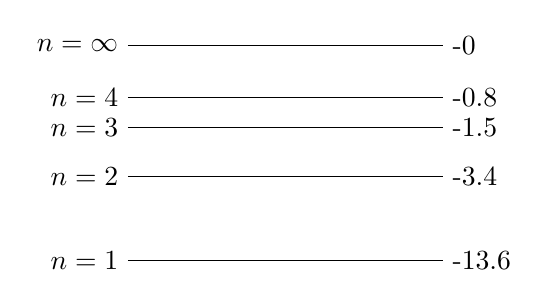
\begin{tikzpicture}
    \foreach \a/\b in {13.6/1,3.4/2,1.5/3,0.8/4,0/\infty} {
        \draw (-2,{6/sqrt(2+\a)}) -- (2,{6/sqrt(2+\a)})
            node[pos=0,anchor=east] {$n=\b$}
            node[pos=1,anchor=west] {\SI{-\a}{\eV}};
    }
\end{tikzpicture}
}

\element{project}{
\begin{question}{testC-Q13}
    %Questions 13 and 14 refer to the following diagram that
    %    gives the energies of some stationary states of hydrogen.
    The following diagram gives the energies of some stationary states of hydrogen.
    \begin{center}
        \hydrogenSpectrum
    \end{center}
    How much energy is emitted when an atom makes a
        transition between the stationary states designated by $n=3$ and $n=2$?
    \begin{multicols}{3}
    \begin{choices}
        \wrongchoice{\SI{1.5}{\eV}}
      \correctchoice{\SI{1.9}{\eV}}
        \wrongchoice{\SI{3.4}{\eV}}
        \wrongchoice{\SI{4.9}{\eV}}
        \wrongchoice{\SI{10.2}{\eV}}
        %% NOTE: add one for eveness
        \wrongchoice{\SI{13.6}{\eV}}
    \end{choices}
    \end{multicols}
\end{question}
}

\element{project}{
\begin{question}{testC-Q14}
    %Questions 13 and 14 refer to the following diagram that
    %    gives the energies of some stationary states of hydrogen.
    The following diagram gives the energies of some stationary states of hydrogen.
    \begin{center}
        \hydrogenSpectrum
    \end{center}
    If hydrogen atoms, as described by the Bohr model,
        are excited to the stationary state designated by $n=3$,
        how many different frequencies of radiation may be emitted by the atoms?
    \begin{multicols}{3}
    \begin{choices}
        \wrongchoice{1}
        \wrongchoice{2}
      \correctchoice{3}
        \wrongchoice{4}
        \wrongchoice{5}
        %% add one for evenness
        \wrongchoice{6}
    \end{choices}
    \end{multicols}
\end{question}
}

\element{project}{
\begin{questionmult}{testC-Q15}
    Which of the following three statements is (are) true of cathode rays?
    \begin{choices}
        \wrongchoice{They are emitted by a variety of cathode materials.}
      \correctchoice{Their paths may be bent by magnetic fields.}
      \correctchoice{Their paths may be bent by electric fields.}
    \end{choices}
\end{questionmult}
}

\element{project}{
\begin{questionmult}{testC-Q16}
    According to classical electromagnetic theory,
        which of the following should occur in an atomic model
        that has electrons revolving in orbits around the nucleus?
    \begin{choices}
      \correctchoice{Electrons should lose energy and fall into the nucleus.}
      \correctchoice{Electrons should emit radiation continually.}
    \end{choices}
\end{questionmult}
}

\element{project}{
\begin{question}{testC-Q17}
    A beam of alpha particles with kinetic energy
        \SI{3}{\mega\eV} is directed at a \emph{gold} foil \num{1 000} atoms thick.
    A second beam of alpha particles with kinetic energy
        \SI{3}{\mega\eV} is directed at a \emph{silver} foil \num{1 000} atoms thick.
    \begin{choices}
        \wrongchoice{The number of a particles scattered back by both foils will be identical.}
      \correctchoice{The number of a particles scattered back by the gold foil will be different from the number scattered back by the silver foil.}
        \wrongchoice{Each foil will scatter all the particles directed at it.}
        \wrongchoice{There will be no scattering by either foil.}
    \end{choices}
\end{question}
}

\element{project}{
\begin{questionmult}{testC-Q18}
    A clean surface of potassium metal will emit
        electrons when exposed to blue light.
    If the intensity of the blue light is increased,
        which of the following will also increase?
    \begin{choices}
      \correctchoice{The number of electrons ejected per second.}
        \wrongchoice{The maximum kinetic energy of the ejected electrons.}
    \end{choices}
\end{questionmult}
}

\element{project}{
\begin{question}{testC-Q19}
    X-rays are:
    \begin{choices}
        \wrongchoice{low-energy cathode rays.}
      \correctchoice{high-energy photons.}
        \wrongchoice{ionized gas molecules.}
        \wrongchoice{waves accompanying photoelectrons.}
        \wrongchoice{particles traveling at speeds just below the speed of light.}
    \end{choices}
\end{question}
}

\element{project}{
\begin{question}{testC-Q20}
    %Question 20 refers to the following diagram.
    A beam of cathode rays traveling between two parallel plates,
        one positively charged and the other negatively charged,
    \begin{center}
    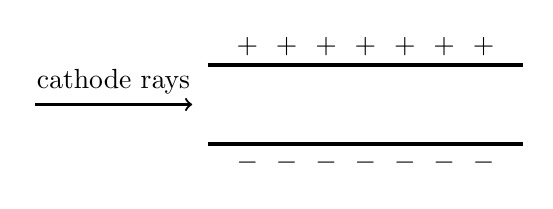
\begin{tikzpicture}
        %% ray
        \draw[thick,<-] (-2.2,0) -- ++(180:2) node[pos=0.5,anchor=south] {cathode rays};
        %% upper plate
        \draw[very thick] (-2,+0.5) -- (2,+0.5);
        \foreach \x in {-1.50,-1.00,-0.5,0,0.5,1.00,1.50} \node[anchor=south] at (\x,0.5) {$+$};
        %% lower plate
        \draw[very thick] (-2,-0.5) -- (2,-0.5);
        \foreach \x in {-1.50,-1.00,-0.5,0,0.5,1.00,1.50} \node[anchor=north] at (\x,-0.5) {$-$};
    \end{tikzpicture}
    \end{center}
    \begin{choices}
      \correctchoice{is deflected towards the positive plate.}
        \wrongchoice{is deflected towards the negative plate.}
        \wrongchoice{is not deflected.}
    \end{choices}
\end{question}
}

\element{project}{
\begin{question}{testC-Q21}
    \ce{CuO} and \ce{CU2O} are two compounds of copper and oxygen.
    If \SI{4}{\gram} of copper combine with \SI{1}{\gram} of oxygen to form \ce{CuO},
        what weight of copper will combine with \SI{1}{\gram} of oxygen to form \ce{Cu2O}?
    \begin{multicols}{3}
    \begin{choices}
        \wrongchoice{\SI{1/4}{\gram}}
        \wrongchoice{\SI{1/2}{\gram}}
        \wrongchoice{\SI{2}{\gram}}
        \wrongchoice{\SI{4}{\gram}}
      \correctchoice{\SI{8}{\gram}}
    \end{choices}
    \end{multicols}
\end{question}
}

\element{project}{
\begin{question}{testC-Q22}
    Mercury vapor, when conducting a current, appears bluish-green.
    What is observed when the light from glowing mercury vapor is analyzed in a spectroscope?
    \begin{choices}
      \correctchoice{a series of discrete lines}
        \wrongchoice{a series of irregular bluish-green flashes}
        \wrongchoice{a bluish-green glow}
        \wrongchoice{the entire visible light spectrum with some dark lines}
    \end{choices}
\end{question}
}

%% NOTE: duplicate of testB-Q14
\element{project}{
\begin{question}{testC-Q23}
    Millikan's charged oil-drop experiment was the first conclusive experimental demonstration that:
    \begin{choices}
      \correctchoice{electric charge is found as multiples of a certain unit charge.}
        \wrongchoice{all electrons have a negative charge.}
        \wrongchoice{electrons are particles.}
        \wrongchoice{electrons have wave properties.}
        \wrongchoice{all atoms contain electrons.}
    \end{choices}
\end{question}
}

\begin{comment}
%% NOTE: TODO: fix formatting
%% NOTE: make vertical instead of horizontal
%% Two colummn, 
%% Rows: Element, Atom, Valence, and Quantity of elemment,
%\newcommand{\testCTable}{
%\begin{tabu}{X[2c]X[c]X[c]X[c]}
%    Element & Hydrogen (C) & Zinc (Zn) & Phosphorus (P) \\
%    Atomic Mass & 1.0 & 65.0 & \\
%    Valence     & 1   & 2    & 3 \\
%    Quantity of element produced by one faraday of charge
%        \SI{1.0}{\gram} & & \SI{10.3}{\gram} \\
%\end{tabu}
%}
\newcommand{\testCTable}{
\begin{tabu}{X[2c]X[c]X[c]X[2c]}
    Element &
    Atomic Mass &
    Valence &
    Quantity of element produced by one faraday of charge \\
    \midrule
    Hydrogen (\ce{H})   &  1.0  & 1 & \SI{1.0}{\gram} \\
    Zinc (\ce{Zn})      & 65.0  & 2 &                 \\
    Phosphorus (\ce{P}) &       & 3 & \SI{10.3}{\gram} \\
\end{tabu}
}

\element{project}{
\begin{question}{testC-Q24}
    %Questions 24 to 26 refer to the following table that gives some data from electrolysis experiments.
    The following table gives some data from electrolysis experiments.
    \begin{center}
        \testCTable
    \end{center}
    The quantity of zinc deposited by one faraday of electric charge is:
    \begin{multicols}{2}
    \begin{choices}
        \wrongchoice{\SI{21.7}{\gram}}
      \correctchoice{\SI{32.5}{\gram}}
        \wrongchoice{\SI{65}{\gram}}
        \wrongchoice{\SI{130}{\gram}}
    \end{choices}
    \end{multicols}
\end{question}
}

\element{project}{
\begin{question}{testC-Q25}
    %Questions 24 to 26 refer to the following table that gives some data from electrolysis experiments.
    The following table gives some data from electrolysis experiments.
    \begin{center}
        \testCTable
    \end{center}
    The atomic mass of phosphorus is:
    \begin{multicols}{2}
    \begin{choices}
        \wrongchoice{3.4}
        \wrongchoice{10.3}
        \wrongchoice{20.6}
      \correctchoice{30.9}
    \end{choices}
    \end{multicols}
\end{question}
}

\element{project}{
\begin{question}{testC-Q26}
    %Questions 24 to 26 refer to the following table that gives some data from electrolysis experiments.
    The following table gives some data from electrolysis experiments.
    \begin{center}
        \testCTable
    \end{center}
    The most obvious formula for a compound of hydrogen and phosphorus is:
    \begin{multicols}{2}
    \begin{choices}
        \wrongchoice{\ce{HP}}
        \wrongchoice{\ce{HP2}}
        \wrongchoice{\ce{HP3}}
      \correctchoice{\ce{H3P}}
        \wrongchoice{\ce{H2P3}}
    \end{choices}
    \end{multicols}
\end{question}
}
\end{comment}

\element{project}{
\begin{question}{testC-Q27}
    Physicists are willing to accept the wave-particle dualism because:
    \begin{choices}
        \wrongchoice{the waves associated with particles are too small to be measured.}
        \wrongchoice{two theories are always better than one.}
      \correctchoice{both wave and particle descriptions are needed to understand experimental results.}
        \wrongchoice{the dualism is confirmed by the theory of relativity.}
    \end{choices}
\end{question}
}

\element{project}{
\begin{question}{testC-Q28}
    Einstein explained the photoelectric effect by assuming that:
    \begin{choices}
        \wrongchoice{the charge of an electron increases with speed.}
        \wrongchoice{atoms do not radiate energy from stationary states.}
        \wrongchoice{the mass of an electron increases with speed.}
      \correctchoice{light consists of quanta of energy,}
        \wrongchoice{the energy of light increases with speed.}
    \end{choices}
\end{question}
}

\element{project}{
\begin{question}{testC-Q29}
    \emph{All except one} of the following are properties of x-rays.
    Which one is the exception?
    \begin{choices}
        \wrongchoice{They penetrate light materials.}
        \wrongchoice{They ionize gases.}
      \correctchoice{They are deflected by magnetic fields.}
        \wrongchoice{They discharge electrified bodies.}
        \wrongchoice{They are diffracted by crystals.}
    \end{choices}
\end{question}
}

%% NOTE: duplicate of testA-Q04
\element{project}{
\begin{question}{testC-Q30}
    A reasonable prediction,
        based on the evolution of previous scientific theories,
        is that in the future the quantum theory will:
    \begin{choices}
        \wrongchoice{be replaced by a theory based on a mechanical model.}
      \correctchoice{be replaced by a more general theory.}
        \wrongchoice{be shown to be wrong.}
        \wrongchoice{explain everything about nature.}
    \end{choices}
\end{question}
}

\element{project}{
\begin{question}{testC-Q31}
    \emph{All except one} of the following are true of an
        electron of rest mass $m_0$ moving with high speed.
    Which one is the exception?
    \begin{choices}
        \wrongchoice{Its mass is greater than $m_0$ .}
        \wrongchoice{Its momentum is greater than $m_0v$.}
        \wrongchoice{It behaves also like a wave train of wavelength $\frac{h}{p}$.}
        \wrongchoice{Its kinetic energy is greater than $\frac{1}{2}m_0v^2$.}
      \correctchoice{Its charge is greater than $q_e$.}
    \end{choices}
\end{question}
}

%% NOTE: near duplicate of testB-Q13
\element{project}{
\begin{question}{testC-Q32}
    The model of the atom used in quantum mechanics is:
    \begin{choices}
        \wrongchoice{the planetary model described by Bohr.}
        \wrongchoice{similar to Bohr's model, but with elliptical orbits for the electrons.}
      \correctchoice{mathematical.}
        \wrongchoice{the ``raisin pudding'' model of electrons dispersed in positive electricity.}
        \wrongchoice{a small solid sphere.}
    \end{choices}
\end{question}
}

\element{project}{
\begin{question}{testC-Q33}
    Bohr dealt with the dilemmas of the planetary model of atoms by:
    \begin{choices}
        \wrongchoice{adjusting the data to fit his theory.}
      \correctchoice{postulating that parts of classical theory did not apply.}
        \wrongchoice{postulating that atoms are unstable.}
        \wrongchoice{postulating that electrons have no energy.}
        \wrongchoice{disproving the Balmer formula.}
    \end{choices}
\end{question}
}

\element{project}{
\begin{question}{testC-Q34}
    The wave-particle dualism of matter can be confirmed experimentally for:
    \begin{multicols}{2}
    \begin{choices}
      \correctchoice{electrons.}
        \wrongchoice{baseballs.}
        \wrongchoice{planets.}
        \wrongchoice{stars.}
        \wrongchoice{water waves.}
    \end{choices}
    \end{multicols}
\end{question}
}

\element{project}{
\begin{question}{testC-Q35}
    The conclusion that the atom has a tiny,
        charged nucleus was first reached from:
    \begin{choices}
        \wrongchoice{the evidence that x-rays can ionize molecules.}
        \wrongchoice{the evidence that x-rays can pass through matter.}
        \wrongchoice{the calculation of the distance between the nucleus and the electron in hydrogen atoms.}
        \wrongchoice{the calculation that 11 series of the hydrogen spectrum are described by the equation
            $\displaystyle {\frac{1}{\lambda} = R_H \left(\frac{1}{n_f^2} - \frac{1}{n_i^2} \right)}$.}
      \correctchoice{the evidence that some $\alpha$ particles are deflected through large angles by thin slices of matter.}
    \end{choices}
\end{question}
}

\element{project}{
\begin{question}{testC-Q36}
    \emph{All except one} of the following are conclusions
        that can be drawn from a quantitative study of electrolysis of water.
    Which one is the exception?
    \begin{choices}
        \wrongchoice{Water is not an element.}
      \correctchoice{Matter has electricity associated with it.}
        \wrongchoice{Hydrogen and oxygen are elements.}
        \wrongchoice{In water, hydrogen and oxygen carry opposite charges.}
    \end{choices}
\end{question}
}

\element{project}{
\begin{question}{testC-Q37}
    %Questions 37 to 39 are statements that relate most directly to one of the following theories.
    %Select the appropriate theory.
    Select the statement that relates most directly to the following theory.
    The mass of a moving object increases as its speed increases.
    \begin{choices}
        \wrongchoice{Bohr's theory}
        \wrongchoice{Heisenberg's uncertainty principle}
        \wrongchoice{Newton's universal theory of gravitation}
      \correctchoice{Einstein's relativity theory}
    \end{choices}
\end{question}
}

\element{project}{
\begin{question}{testC-Q38}
    Select the statement that relates most directly to the following theory.
    There is a limit to the accuracy of the simultaneous
        measurement of the velocity and position of a moving electron.
    \begin{choices}
        \wrongchoice{Bohr's theory}
      \correctchoice{Heisenberg's uncertainty principle}
        \wrongchoice{Newton's universal theory of gravitation}
        \wrongchoice{Einstein's relativity theory}
    \end{choices}
\end{question}
}

\element{project}{
\begin{question}{testC-Q39}
    Select the statement that relates most directly to the following theory.
    The angular momentum of an electron in a hydrogen atom can
        have only the values $\dfrac{h}{2\pi}$, $\dfrac{2h}{2\pi}$, $\dfrac{3h}{2\pi}$.
    \begin{choices}
      \correctchoice{Bohr's theory}
        \wrongchoice{Heisenberg's uncertainty principle}
        \wrongchoice{Newton's universal theory of gravitation}
        \wrongchoice{Einstein's relativity theory}
    \end{choices}
\end{question}
}

\element{project}{
\begin{question}{testC-Q40}
    The Franck-Hertz experiment on the energy of electrons after
        passing through a gas provided evidence for the concept of:
    %% NOTE: mercury atoms can only absorb discrete amounts of momenta
    \begin{choices}
      \correctchoice{discrete atomic energy levels.}
        \wrongchoice{momentum of photons.}
        \wrongchoice{a plum pudding atom.}
        \wrongchoice{Compton scattering.}
        \wrongchoice{electron wavelengths.}
    \end{choices}
\end{question}
}

\endinput

